%!Tex Root = ../Tutorat4.tex
% ./Packete.tex
% ./Design.tex
% ./Deklarationen.tex
% ./Aufgabe1.tex
% ./Aufgabe2.tex
% ./Aufgabe3.tex
% ./Bonus.tex

\section{Appendix}

\subsection{Old Overview}

\begin{frame}{Overview periodic Task Scheduling}
  \centering
  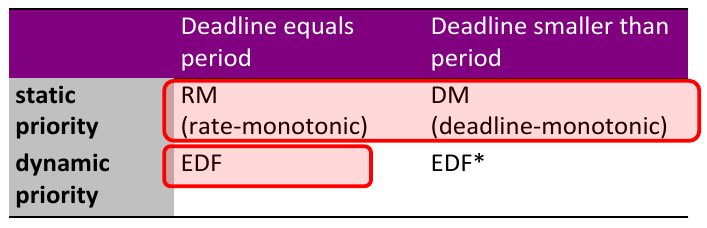
\includegraphics[width=\textwidth]{./figures/overview_real_time_scheduling.png}
\end{frame}

\begin{frame}[shrink=20]{Overview Aperiodic Task Scheduling}{Schedulability test\vspace{0.5cm}}
    \begin{NiceTabular}{X[1,l]X[2,l]X[2,l]}[rules/color=PrimaryColor] % {\linewidth}{|C|C|L|L|}
    \CodeBefore
    \chessboardcolors{white}{BoxColor}
    \rowcolor{PrimaryColor}{1}
    \columncolor{PrimaryColor}{1}
    \Body
    & \textcolor{white}{Deadline equals period ($D_i = T_i$)} & \textcolor{white}{Deadline smaller than period ($D_i \le T_i$)} \\
      \textcolor{white}{static priority} & (1) $\displaystyle\sum_{i=1}^n \frac{C_i}{T_i} \leq n\left(2^{1 / n}-1\right)$ \hspace{2cm} (\alert{sufficient} but \alert{not necessary}) \hspace{2cm}(2) same as Schedulability Test 2 for DM & (1) $\displaystyle\sum_{i=1}^n \frac{C_i}{D_i} \leq n\left(2^{1 / n}-1\right)$ \hspace{2cm} (\alert{sufficient} but \alert{not necessary}) \hspace{2cm} (2) smallest $R_i$ that satisfies $\displaystyle R_i=C_i+\sum_{j=1}^{i-1}\left[\frac{R_i}{T_j}\right] C_j$ and $R_i \le D_i$ for all tasks $\tau_i$ \hspace{3cm} (\alert{necessary} and \alert{sufficient}) \\
    \textcolor{white}{dynamic priority} & $\displaystyle\sum_{i=1}^n \frac{C_i}{T_i}=U \leq 1$ \hspace{2cm} (\alert{necessary} and \alert{sufficient}) & $\rightarrow$ \cite{buttazzo2011hard} \\
    \bottomrule
  \end{NiceTabular}
\end{frame}

\begin{frame}{Mixed Task Sets}{}
    \begin{itemize}
        \item So far: we differentiated between \alert{periodic} and \alert{aperiodic} tasks.
        \item Now: Consider a \alert{mixed} task set!
        \item We want to be able to find a schedule when there's both \alert{periodic} and \alert{aperiodic} tasks.
    \end{itemize}
\end{frame}

\begin{frame}{Schedulability tests}{Sufficient? Necesarry?}
    \begin{itemize}
        \item We're interested in whether a given problem can be scheduled by algorithms.
        \item Depending on the algorithm we can derive sufficient and necesarry conditions.
        \item[]\alert{Sufficient:} If $A \implies B$ then A is a sufficient condition for B.
        \item[]\alert{Necesarry:} If $B \implies A$ then A is a necesarry condition for B.
        \item A necesarry and sufficient condition means, both statements are logically equivalent.
    \end{itemize}
\end{frame}
\begin{frame}{Schedulability tests}{Utilization}
    Different kind of utilizations also play a big role in our analysis. We introduced the \alert{processor utilization factor} $U = \sum\limits_{i=1}^{n}\cfrac{C_i}{T_i}$ and later on $U_s$ as the server utilization.

    (More about servers later)
\end{frame}
\begin{frame}{RM - Rate Monotonic Scheduling}{Schedulability}
\begin{itemize}
    \item RM is optimal among all fixed-priority assignments in the sense that no other fixed-priority algorithm can schedule a task set that cannot be scheduled by RM.
    \item As in the lecture, we have $\sum\limits_{i=1}^{n}\cfrac{C_i}{T_i} \leq n(2^{1/n}-1)$ as a \alert{sufficient} but not \alert{necesarry} condition.
\end{itemize}
\end{frame}
\begin{frame}{RM(PS) - Rate Monotonic Polling Server}
    \begin{itemize}
        \item One way to handle both periodic and aperiodic tasks is to use a so called server.
        \item This PS (Polling Server) acts as a periodic task (meaning it is instantiated at regular intervals $T_s$) whose job it is to, once it has the highest priority, serve any pending aperiodic requests within the limits of a server capacity $C_s$.
        \item Since we introduce yet another periodic task, the schedulability analysis simply is the same as normal $RM$ with one additional task. Again, we have the \alert{sufficient} but not \alert{necesarry} condition: $\cfrac{C_s}{T_s} + \sum\limits_{i=1}^{n}\cfrac{C_i}{T_i} \leq (n+1)(2^{1/(n+1)}-1)$
    \end{itemize}
\end{frame}

% \begin{frame}{EDF - Total Bandwidth Server}
%
% \end{frame}


% \begin{frame}{Overview Aperiodic Task Scheduling}
%   \begin{itemize}
%     \item \alert{Lateness:} $L_i = f_i - d_i$
%     \item \alert{Maximum lateness:} $\displaystyle L_{\max }=\max_i\left(f_i-d_i\right)$
%     \begin{itemize}
%       \item this a a metric to compare schedules
%     \end{itemize}
%   \end{itemize}
% \end{frame}
% %
% \begin{frame}{TT Cyclic Executive Scheduling}{Recap: Definitions}
%     \begin{itemize}
%         \item $\Gamma:$ set of all periodic tasks
%         \item $\tau_i:$ one particular periodic task (the i-th)
%         \item $\tau_{i,j}:$ the $j$th instance of task $i$
%         \item $r_{i,j}:$ release time of $j$th instance of task $i$
%         \item $d_{i,j}:$ absolute deadline of the $j$th instance of task $i$
%         \item $\Phi_i:$ phase of task $i$
%         \item $D_i:$ relative deadline of task $i$
%     \end{itemize}
% \end{frame}
%
% \begin{frame}{TT Cyclic Executive Scheduling}{Recap: Three assumptions}
% \begin{enumerate}
%     \item The instances of a periodic task are regularly activated at a constant rate. The interval between two consecutive activations is called period. The release times satisfy $r_{i,j} = \Phi_i + (j-1)T_i$
%     \item All instances have the same worst case execution time $C_i$ (also written as $WCET(i)$)
%     \item All instances of a periodic task have the same relative deadline $D_i$. Therefore the absolute deadlines satisfy $d_{i,j} = \Phi_i + (j-1)T_i + D_i$
% \end{enumerate}
% \end{frame}
